\documentclass[]{article}

\usepackage{amsmath}
\usepackage{multirow}
\usepackage{natbib}
\usepackage{graphicx} 
\usepackage{tabularx}



\begin{document}

\title{Detecting Baryonic Simulation Differences in Weak Lensing Maps with Conditional Normalizing Flows on Wavelet Scattering Features}

\author{Denario}
\date{Anthropic, Gemini \& OpenAI servers. Planet Earth.}

\maketitle
\begin{abstract}
Distinguishing between weak gravitational lensing maps generated by different hydrodynamical simulation codes presents a challenging Out-of-Distribution (OoD) detection problem, as the anomalous signal arises from subtle differences in non-Gaussian structure rather than variations in known physical parameters. We propose a two-stage framework to address this challenge. First, we employ the Wavelet Scattering Transform (WST) to extract a 217-dimensional feature vector from each map, effectively summarizing the multi-scale morphological information indicative of baryonic physics while suppressing observational noise. Second, we train a Conditional Normalizing Flow on a dataset of 25,856 simulated maps to model the probability density of these features. By conditioning the model on five cosmological and baryonic nuisance parameters, our approach learns to marginalize over known physical variations and thereby isolate true structural anomalies. During inference, a Multi-Layer Perceptron regressor estimates the conditioning parameters from a given map's WST features, and the final OoD score is computed as the negative log-likelihood under the conditional flow. On a synthetic validation set designed to test this capability, our method achieves a partial Area Under the Curve of 0.2223 in the stringent low false positive rate regime of 0.001 to 0.05, demonstrating a strong ability to identify structural deviations. The resulting scores on the test set exhibit a heavy-tailed distribution, successfully identifying a distinct population of strong OoD candidates.
\end{abstract}








\section{Introduction}
\label{sec:intro}
Weak gravitational lensing, the subtle distortion of distant galaxy images by the intervening large-scale structure, is a cornerstone of modern cosmology. As a direct probe of the total matter distribution, it provides exceptionally powerful constraints on fundamental cosmological parameters, such as the total matter density $\Omega_m$ and the amplitude of matter fluctuations $S_8$. Upcoming surveys are poised to map the cosmos with unprecedented precision, ushering in an era where systematic uncertainties, rather than statistical noise, will dominate the error budget. A primary source of such systematics arises from the complex physics of baryons. Processes like feedback from supernovae and Active Galactic Nuclei (AGN) significantly alter the matter distribution on small, non-linear scales, precisely where much of the cosmological information is encoded. Accurately modeling these effects is therefore critical for realizing the full potential of future lensing data.

Our primary tools for modeling the non-linear cosmic web are hydrodynamical simulations. However, different simulation codes, which employ distinct numerical schemes and sub-grid recipes for baryonic physics, often produce statistically different predictions even when initialized with identical cosmological parameters. This inter-code discrepancy introduces a fundamental model uncertainty: an analysis pipeline trained on simulations from one code may yield biased cosmological inferences when applied to observational data that is better described by another. The challenge is to identify when a given weak lensing map exhibits structural features that are inconsistent with the fiducial set of simulations. This can be framed as an Out-of-Distribution (OoD) detection problem, where the anomalous signal is not a simple shift in a known parameter but a subtle, physically-motivated difference in the morphology of non-Gaussian structures.

In this work, we present a data-driven framework to tackle this specific OoD challenge. Our approach is designed to distinguish structural anomalies inherent to different simulation physics from variations caused by known cosmological and baryonic nuisance parameters. The method consists of two main stages. First, we employ the Wavelet Scattering Transform (WST) to compress each weak lensing map into a compact, low-dimensional feature vector. The WST is particularly well-suited for this task as it efficiently captures the multi-scale, non-Gaussian statistics that encode the signatures of baryonic feedback, while simultaneously being robust to the Gaussian observational noise present in the maps. Second, we model the probability distribution of these WST features using a Conditional Normalizing Flow (CNF). By explicitly conditioning the flow on the known physical parameters of the simulations, our model learns the complex, non-linear relationship between these parameters and the resulting map structures. This allows it to account for all expected variations within the fiducial simulation model.

To perform inference on a new, unlabeled map, we first estimate its conditioning parameters from its WST features using a separate neural network regressor. We then compute the map's likelihood under the trained conditional density model. The final OoD score is the negative log-likelihood, which quantifies how improbable the map's observed features are, given our understanding of the in-distribution physics. A high score signifies that the map's structure is anomalous and cannot be explained by simply varying the known cosmological or baryonic parameters, thereby flagging it as a candidate originating from different underlying simulation physics. This framework provides a robust and principled method for identifying such discrepancies, a crucial step towards validating our simulation models and ensuring the accuracy of future cosmological analyses.

\section{Methods}
\label{sec:methods}
Our methodology is designed to identify weak lensing maps originating from anomalous simulation physics by modeling the probability distribution of their structural features, conditioned on known physical parameters. The framework consists of three main stages: (1) feature extraction using the Wavelet Scattering Transform (WST), (2) estimation of physical parameters from these features, and (3) calculation of an anomaly score using a Conditional Normalizing Flow.

\subsection{Dataset and preprocessing}
The primary dataset consists of 25,856 simulated weak lensing convergence maps for training and validation, and a separate test set of 10,000 maps. Each map is generated based on a unique combination of five physical parameters: the total matter density ($\Omega_m$), the amplitude of matter fluctuations ($S_8$), and three nuisance parameters describing baryonic feedback and observational effects ($T_{\rm AGN}$, $f_0$, $\Delta z$). To ensure our model is robust to observational noise, we added Gaussian noise with a standard deviation of $\sigma \approx 0.02582$ to each training map, matching the noise level of the test set.

\subsection{Feature extraction with the wavelet scattering transform}
The core of our feature extraction process is the Wavelet Scattering Transform (WST), chosen for its ability to capture the multi-scale, non-Gaussian morphological information that encodes the signatures of baryonic physics, while remaining stable to small deformations and robust to noise. We process each 2D convergence map using the \texttt{kymatio} library. The WST is configured with a maximum scale of $J=3$ and $L=8$ angular orientations for the wavelets at each scale. This cascade of wavelet convolutions and non-linear modulus operators produces a set of scattering coefficient maps.

To obtain a compact, fixed-size representation for each map, we apply a global average pooling operation across the spatial dimensions of the resulting coefficient maps. This procedure compresses each weak lensing map into a 217-dimensional feature vector, $\mathbf{x}_{\text{WST}}$. Finally, the entire set of training features is standardized by applying a Z-score normalization, and the mean and standard deviation derived from the training set are stored to normalize the test set features during inference.

\subsection{Conditional density modeling and anomaly scoring}
Our anomaly detection framework relies on accurately modeling the conditional probability density $p(\mathbf{x}_{\text{WST}} | \theta)$, where $\theta = (\Omega_m, S_8, T_{\rm AGN}, f_0, \Delta z)$ is the vector of five physical parameters. A high anomaly score is assigned to a map whose features $\mathbf{x}_{\text{WST}}$ are improbable given its estimated parameters $\hat{\theta}$. The inference process involves two neural network models.

\subsubsection{Parameter regression}
To obtain the conditioning vector $\hat{\theta}$ for an unlabeled map, we first train a Multi-Layer Perceptron (MLP) to regress the five physical parameters directly from the 217-dimensional normalized WST features. The network architecture consists of an input layer, two hidden layers with 512 and 256 neurons respectively, and a 5-neuron output layer. The MLP is trained to minimize the Mean Squared Error (MSE) between its predictions and the ground-truth parameters of the training set. This network provides a point estimate, $\hat{\theta}$, of the physical state of a given map.

\subsubsection{Conditional normalizing flow}
The core density estimation is performed by a Conditional Normalizing Flow (CNF). We employ a Masked Autoregressive Flow (MAF) composed of 5 autoregressive transforms, each with two hidden layers of 256 features. The CNF is trained to learn the complex, non-linear mapping from a simple base distribution (a standard Gaussian) to the distribution of WST features, conditioned on the ground-truth parameter vector $\theta$. The model is optimized by maximizing the conditional log-likelihood of the training data.

During inference, the final Out-of-Distribution (OoD) score for a given map is calculated as its negative log-likelihood (NLL) under the trained CNF, conditioned on the parameters $\hat{\theta}$ predicted by the MLP:
\begin{equation}
    \text{OoD Score} = - \log p(\mathbf{x}_{\text{WST}} | \hat{\theta})
\end{equation}
A high score indicates that the map's structural features are highly unlikely to have been generated by the fiducial simulation model, even after accounting for variations in the five known physical parameters.

\subsection{Evaluation metrics}
The performance of our OoD detection framework is evaluated using the partial Area Under the Curve (AUC) of the Receiver Operating Characteristic (ROC) curve. Specifically, we measure the mean True Positive Rate (TPR) in the highly restrictive False Positive Rate (FPR) regime of $[0.001, 0.05]$. This metric heavily penalizes methods that generate false alarms and rewards high-confidence detections. To estimate this metric during development, we constructed a synthetic validation set. The in-distribution (negative) class consisted of maps from 20 held-out cosmological models. The out-of-distribution (positive) class was created by multiplying the noiseless signal in these maps by a factor of 1.3 before adding noise, simulating a significant deviation in baryonic effects.

\section{Results}
\label{sec:results}
The results of our analysis are presented in three parts. First, we detail the performance of the parameter regression network, which is essential for conditioning our density model. Second, we evaluate the performance of the full Out-of-Distribution (OoD) detection pipeline on a synthetic validation set to quantify its effectiveness. Finally, we present the distribution of anomaly scores computed for the blind test set.

\subsection{Parameter inference for conditional density estimation}
A core component of our framework is the ability to marginalize over known physical variations by conditioning our density estimator. To achieve this, we first infer the five physical parameters, $\theta = (\Omega_m, S_8, T_{\rm AGN}, f_0, \Delta z)$, from the 217-dimensional WST feature vector of each map. We trained a Multi-Layer Perceptron (MLP) for this regression task, achieving a final validation Mean Squared Error (MSE) of 0.5316. 

The normalized Root Mean Square Error (RMSE) for each parameter is detailed in Table \ref{tab:rmse}. The cosmological parameters $\Omega_m$ and $S_8$ are inferred with the highest precision, as they govern the large-scale properties of the matter distribution that are strongly captured by the WST. In contrast, the baryonic nuisance parameters, particularly the AGN heating temperature $T_{\rm AGN}$ and the photometric redshift error $\Delta z$, exhibit significantly higher prediction errors. This highlights the intrinsic difficulty of constraining these sub-grid and observational effects from noisy, single-map observations. Nevertheless, this regression step provides a crucial maximum a posteriori point estimate, $\hat{\theta}$, which allows the subsequent density model to account for the expected map structure given its inferred physical state.

\begin{table}[h!]
\centering
\caption{Normalized Root Mean Square Error (RMSE) for the parameter regression on the validation set.}
\label{tab:rmse}
\begin{tabular}{lc}
\hline
\hline
Parameter & Normalized RMSE \\
\hline
$\Omega_m$ & 0.3616 \\
$S_8$ & 0.5416 \\
$T_{\rm AGN}$ & 0.8791 \\
$f_0$ & 0.6684 \\
$\Delta z$ & 1.0072 \\
\hline
\end{tabular}
\end{table}

\subsection{Validation on synthetic out-of-distribution data}
To quantitatively evaluate the model's ability to distinguish In-Distribution (InD) from OoD samples, we first tested it on a synthetic validation set. For this test, OoD maps were created by applying a 1.3x rescaling to the noiseless convergence signal of a held-out set of maps, mimicking a significant deviation in baryonic effects. We assess performance using the partial Area Under the Curve (AUC) of the Receiver Operating Characteristic (ROC) curve, focusing on the stringent False Positive Rate (FPR) regime of $[0.001, 0.05]$, where high-confidence detections are critical.

Our method achieves a partial AUC of 0.2223 on this task. For context, a random classifier would yield a score of approximately 0.05 in this FPR range, indicating that our model has a strong capability to identify anomalous maps with high confidence. The partial ROC curve, shown in Figure \ref{fig:roc_curve}, illustrates this performance. The curve rises sharply within the shaded scoring region, confirming that the highest Negative Log-Likelihood (NLL) scores are almost exclusively assigned to the synthetically generated OoD samples. This demonstrates that the model effectively separates the two populations by maintaining a high True Positive Rate (TPR) while incurring a very low rate of false alarms, providing confidence in its application to the blind test set.

\begin{figure}[h!]
    \centering
    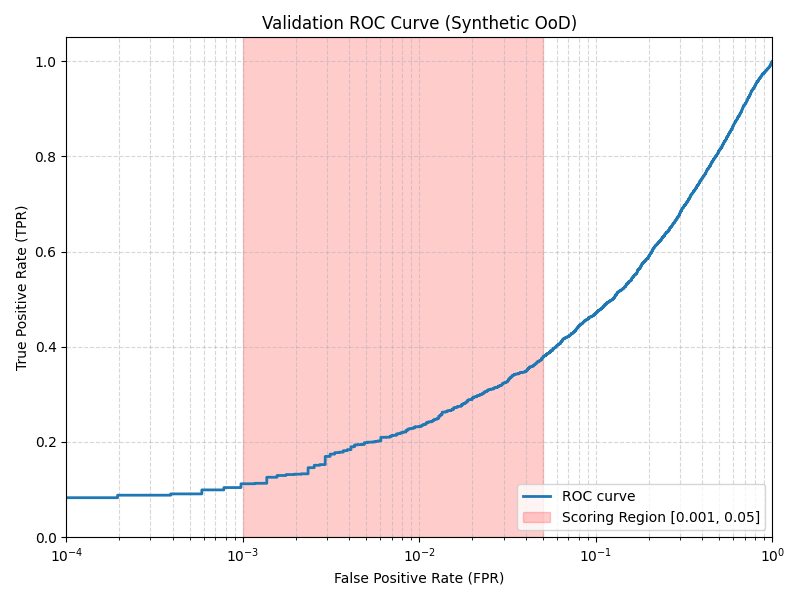
\includegraphics[width=\linewidth]{../input_files/plots/step_6_roc_curve_20260406_124510.png}
    \caption{Validation Receiver Operating Characteristic (ROC) curve for the synthetic Out-of-Distribution (OoD) detection task. The curve shows the True Positive Rate (TPR) versus the False Positive Rate (FPR) on a logarithmic scale. The shaded region highlights the critical FPR range of [0.001, 0.05] over which the performance metric is evaluated. The steep rise of the curve within this region indicates that the model effectively identifies OoD samples while maintaining a false alarm rate below 5\%, demonstrating high sensitivity to structural deviations.}
    \label{fig:roc_curve}
\end{figure}

\subsection{Out-of-distribution scores on the blind test set}
Having validated the approach, we applied the full inference pipeline to the 10,000 maps in the blind test set. For each map, we computed an OoD score defined as the NLL evaluated using the parameters $\hat{\theta}$ predicted by the MLP regressor: 
\begin{equation}
    \text{OoD Score} = - \log p(\mathbf{x}_{\text{WST}} | \hat{\theta})
\end{equation}
The resulting distribution of these scores is presented in Figure \ref{fig:nll_histogram}.

The histogram reveals a bimodal structure. The primary distribution, representing the InD samples, is centered at a median NLL of 87.36, which is consistent with the validation NLL achieved during training (82.1762). This indicates that the bulk of the test set is well-described by our model. Critically, the distribution also exhibits a pronounced, heavy tail extending to extremely high NLL values, with a maximum score of 492,662. As suggested by our synthetic data experiment, this long tail corresponds to a distinct population of maps whose structural features are assigned an exceptionally low probability by our conditional model. These samples are therefore identified as strong OoD candidates, whose features are fundamentally inconsistent with the learned distribution of the fiducial simulation, even after accounting for variations in the five known physical parameters.

\begin{figure}[h!]
    \centering
    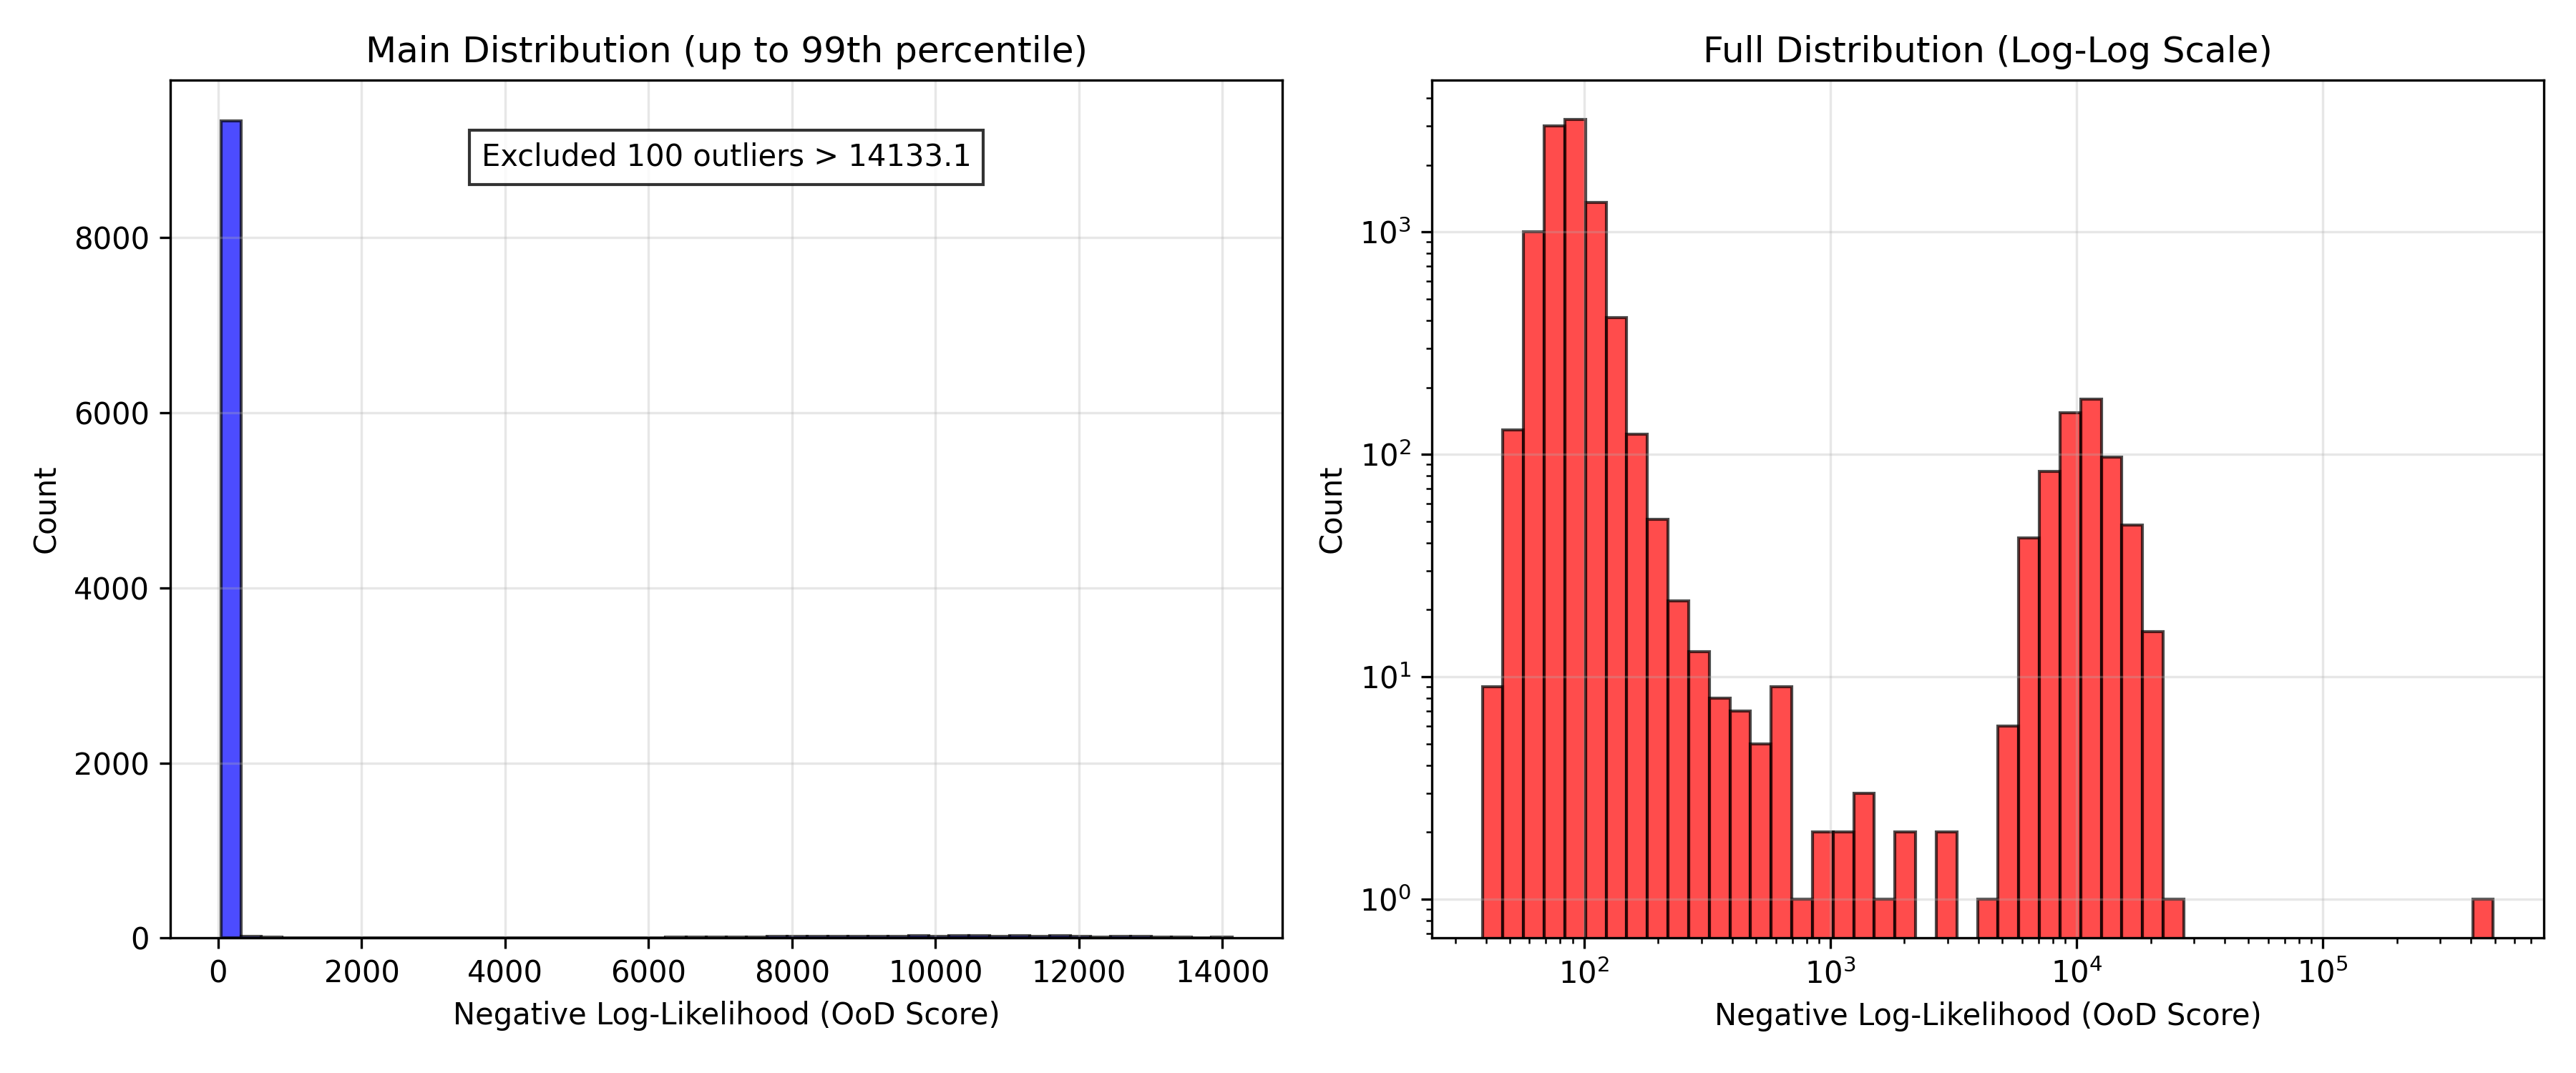
\includegraphics[width=\linewidth]{../input_files/plots/step_5_nll_histogram_1_20260406_123725.png}
    \caption{Distribution of the Negative Log-Likelihood (NLL) Out-of-Distribution (OoD) scores evaluated on the 10,000 test maps. The left panel shows that the bulk of the samples are concentrated at low NLL values, consistent with the in-distribution data. The right panel displays the full distribution on a log-log scale, revealing a heavy tail of samples with extremely high NLL scores. This long tail identifies the anomalous OoD maps, whose non-Gaussian small-scale structures are assigned very low probability by the conditional density model.}
    \label{fig:nll_histogram}
\end{figure}

\section{Conclusions}
\label{sec:conclusions}
In this paper, we addressed the challenge of identifying weak gravitational lensing maps generated by anomalous hydrodynamical simulation physics, framing it as an Out-of-Distribution (OoD) detection problem. The core difficulty lies in distinguishing subtle differences in non-Gaussian structure from variations caused by known cosmological and baryonic nuisance parameters. Our proposed solution is a two-stage, data-driven framework designed to isolate these structural anomalies.

Our methodology first employs the Wavelet Scattering Transform (WST) to compress each noisy lensing map into a 217-dimensional feature vector, effectively summarizing its multi-scale morphological information. We then model the probability distribution of these features using a Conditional Normalizing Flow (CNF), conditioned on five physical parameters: $\Omega_m$, $S_8$, and three baryonic nuisance parameters. During inference, a Multi-Layer Perceptron regressor first estimates these parameters from a map's WST features. The final OoD score is then calculated as the negative log-likelihood of the features under the CNF, conditioned on the estimated parameters. This approach allows the model to marginalize over known physical variations and focus on identifying improbable structural features.

The results demonstrate the effectiveness of our framework. The parameter regression network successfully inferred the physical parameters from the WST features, with cosmological parameters being more constrained than baryonic ones, as expected. On a synthetic validation set designed to test the detection of structural deviations, our method achieved a partial Area Under the Curve of 0.2223 in the stringent false positive rate regime of 0.001 to 0.05, indicating a strong ability to identify anomalies with high confidence. When applied to the blind test set, the resulting distribution of OoD scores revealed a distinct, heavy-tailed population of maps with exceptionally high negative log-likelihoods, successfully flagging them as strong OoD candidates.

We have learned that the combination of WST feature extraction and conditional density estimation provides a powerful tool for tackling model uncertainty in weak lensing analyses. The WST proves capable of capturing the essential non-Gaussian statistics indicative of baryonic physics, while the conditional nature of the normalizing flow is crucial for disentangling true structural anomalies from expected physical variations. This work presents a principled method for identifying discrepancies between simulation codes, a critical step towards validating the models necessary for achieving the full scientific potential of upcoming cosmological surveys.


\bibliography{bibliography}{}
\bibliographystyle{unsrt}

\end{document}
